\section{Square Class Reference}
\label{classSquare}\index{Square@{Square}}
Inheritance diagram for Square::\begin{figure}[H]
\begin{center}
\leavevmode
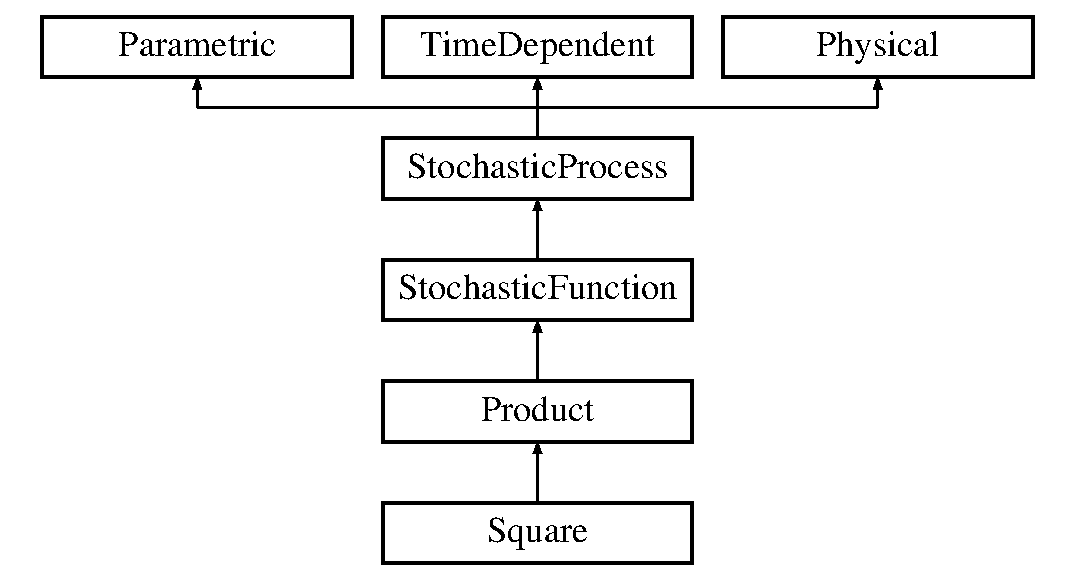
\includegraphics[height=5cm]{classSquare}
\end{center}
\end{figure}


\subsection{Detailed Description}
returns the product of Xt$\ast$Xt and a scalar \subsection*{Public Member Functions}
\begin{CompactItemize}
\item 
virtual double {\bf calculateNextValue} ()\label{classSquare_b03010f31f1716e6ca06c05ad2442c95}

\begin{CompactList}\small\item\em Returns the value at the next time step. \item\end{CompactList}\item 
virtual double {\bf calculateCurrentValue} ()\label{classSquare_1235e02863dad7becef8e8fe04050e66}

\begin{CompactList}\small\item\em Returns the value at the current time step. \item\end{CompactList}\end{CompactItemize}
